\documentclass[compress]{beamer}

\usepackage[T1]{fontenc}
\usepackage[utf8]{inputenc}
\usepackage[catalan]{babel}
\usepackage{lmodern}

\mode<presentation>
{
	\usetheme{Singapore}
	\usecolortheme{lily}

	\setbeamertemplate{footline}[frame number]
	\setbeamertemplate{navigation symbols}{}
}

\usepackage{graphicx}
\usepackage{booktabs}
\usepackage{multicol}

\usepackage[amssymb]{SIunits}
\usepackage{listings}
\lstloadlanguages{VHDL, C, bash}
	\lstset
	{
		language=C, %-> choose the language of the code
		%basicstyle=\scriptsize,% -> the size of the fonts used for the code
		basicstyle=\tiny,% -> the size of the fonts used for the code
		numbers=none,% -> where to put the line-numbers
		numberstyle=\tiny,% -> size of the fonts used for the line-numbers
		stepnumber=1,% -> the step between two line-numbers.
		numbersep=10pt,% -> how far the line-numbers are from the code
		% backgroundcolor=\color[rgb]{0.95, 0.95, 0.95},% -> sets background color (needs package)
		showspaces=false,% -> show spaces adding particular underscores
		showstringspaces=false,% -> underline spaces within strings
		showtabs=false,% -> show tabs within strings through particular underscores
		% frame=single,% -> adds a frame around the code
		tabsize=1,% -> sets default tab-size to 2 spaces
		captionpos=t,% -> sets the caption-position to top
		breaklines=true,% -> sets automatic line breaking
		breakatwhitespace=true,% -> automatic breaks happen at whitespace
		keywordstyle=\color{blue},
		linewidth=\textwidth,
		xleftmargin=0\textwidth,
		xrightmargin=0\textwidth,
		morekeywords={define, byte, millis, map, analogRead, delay, boolean},
		extendedchars=true,
		commentstyle={\color[rgb]{0.1,0.5,0.1}}
	}

% TEST AREA
%Definici� de la ela geminada per tal que accepti el punt volat del teclat
\def�#1{%
  \ifmmode
    \cdot #1
    %\csname normal@char\string"\endcsname l%
  \else%
    \def\argument{#1}%
    \if\argument l%
      \leftllkern=0pt\rightllkern=0pt\raiselldim=0pt%
      \setbox0\hbox{l}\setbox1\hbox{l\/}\setbox2\hbox{.}%
      \advance\raiselldim by \the\fontdimen5\the\font
      \advance\raiselldim by -\ht2%
      \leftllkern=-.25\wd0%
      \advance\leftllkern by \wd1%
      \advance\leftllkern by -\wd0%
      \rightllkern=-.25\wd0%
      \advance\rightllkern by -\wd1%
      \advance\rightllkern by \wd0%
      \allowhyphens\discretionary{-}{l}%
      {\hbox{}\kern\leftllkern\raise\raiselldim\hbox{.}%
        \kern\rightllkern\hbox{l}}\allowhyphens%
    \else
      \if\argument L%
        \leftllkern=0pt\rightllkern=0pt\raiselldim=0pt%
        \setbox0\hbox{L}\setbox1\hbox{L\/}\setbox2\hbox{.}%
        \advance\raiselldim by .5\ht0%
        \advance\raiselldim by -.5\ht2%
        \leftllkern=-.125\wd0%
        \advance\leftllkern by \wd1%
        \advance\leftllkern by -\wd0%
        \rightllkern=-\wd0%
        \divide\rightllkern by 6%
        \advance\rightllkern by -\wd1%
        \advance\rightllkern by \wd0%
        \allowhyphens\discretionary{-}{L}%
        {\hbox{}\kern\leftllkern\raise\raiselldim\hbox{.}%
           \kern\rightllkern\hbox{L}}\allowhyphens%
      \else
        #1
      \fi
    \fi
  \fi
  }
% TEST AREA

% TITLE PAGE
	\title{An\`alisi de la interconnexi\'o de dispositius\\l\`ogics programables mitjan\c cant Ethernet}
	\author{Marko Peshevski}
	\institute{TFM, MUESAEI}
	\date{Q1 2016 -- 2017}
% TITLE PAGE

\begin{document}

\begin{frame}[plain]
	\titlepage
\end{frame}

\begin{frame}
    \frametitle{Taula de continguts}
    \begin{multicols}{2}
    \tableofcontents
    \end{multicols}
\end{frame}

\setcounter{framenumber}{0}
\section{Introducci\'o}
	\subsection{Objectius}
		\begin{frame}
			\frametitle{Objectius}
				\begin{itemize}
					\item{Con\`eixer Ethernet en profunditat}
					\item{Con\`eixer en profunditat alguns protocols de xarxes}
					\item{Desenvolupar un sistema incrustat amb Ethernet sobre una FPGA}
					\item{Intentar desenvolupar una pila de protocol b\`asica}
				\end{itemize}
		\end{frame}

\section{FPGA}
	\subsection{Estructura}
		\begin{frame}
			\frametitle{Estructura}
			\framesubtitle{}
				\begin{itemize}
					\item{Matriu de blocs l\`ogics, interconnectats}
					\item{Recursos d'interconnexi\'o}
					\item{Blocs d'entrada/sortida}
				\end{itemize}
				\begin{figure}
					\includegraphics[keepaspectratio = true, width=0.4\textwidth]{figures/fig29-1.jpg}
				\end{figure}
		\end{frame}

		\begin{frame}
			\frametitle{Estructura}
			\framesubtitle{Blocs l\`ogics}
				\begin{itemize}
					\item{Taules d'entrada (Look Up Table)}
					\item{L\`ogica operativa per c\`alculs}
					\item{Multiplexors}
					\item{Biestables s\'incrons}
				\end{itemize}
				\begin{figure}
					\includegraphics[keepaspectratio = true, width=0.9\textwidth]{figures/FPGA_cell_example.png}
				\end{figure}
		\end{frame}

		\begin{frame}
			\frametitle{Estructura}
			\framesubtitle{Recursos d'interconnexi\'o}
				\begin{itemize}
					\item{Permeten encaminar les connexions entre blocs l\`ogics i blocs d'entrada/sortida}
					\item{Es tria l'estat dels interruptors al programar la FPGA}
				\end{itemize}
				\begin{figure}
					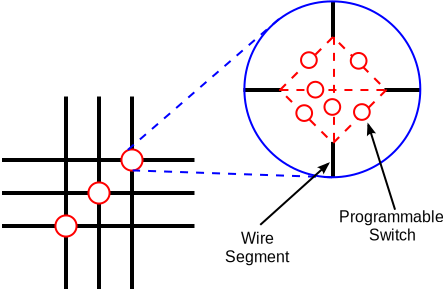
\includegraphics[keepaspectratio = true, width=0.5\textwidth]{figures/Switch_box.png}
				\end{figure}
		\end{frame}

		\begin{frame}
			\frametitle{Estructura}
			\framesubtitle{Blocs d'entrada/sortida}
				\begin{itemize}
					\item{Biestables s\'incrons}
					\item{Control tri-estat: entrada, sortida o alta imped\`ancia}
					\item{Connexi\'o amb el m\'on exterior}
				\end{itemize}
				\begin{figure}
					\includegraphics[keepaspectratio = true, width=0.7\textwidth]{figures/slide_21.png}
				\end{figure}
		\end{frame}

	\subsection{Nuclis de propietat inte\l.lectual}
		\begin{frame}
			\frametitle{Nuclis de propietat intel�lectual}
			\framesubtitle{}
				\begin{itemize}
					\item{Implementacions en llenguatge de descripci\'o de hardware (principalment VHDL o Verilog)}
					\item{Generalment anomenats soft-cores}
					\item{Existeixen els hard-cores, incrustats sobre el silici de la FPGA}
					\item{Exemples variats: perif\`eric SPI, microcontrolador sencer (MicroBlaze de Xilinx), convertidor digital-anal\`ogic, \ldots}
				\end{itemize}
		\end{frame}

		\begin{frame}
			\frametitle{Nuclis de propietat intel�lectual}
			\framesubtitle{Disseny de hardware}
				\begin{itemize}
					\item{Cada fabricant ofereix les seves eines per generar hardware}
					\item{En el cas de Xilinx, la eina \'es el Xilinx Platform Studio}
				\end{itemize}
				\begin{figure}
					\includegraphics[keepaspectratio = true, width=0.6\textwidth]{figures/vista_config_xps.png}
				\end{figure}
				\begin{itemize}
					\item{Un cop creat el hardware, si hi ha un microcontrolador o microprocessador s'ha de programar}
				\end{itemize}
		\end{frame}

		\begin{frame}
			\frametitle{Nuclis de propietat intel�lectual}
			\framesubtitle{Programaci\'o de software}
				\begin{itemize}
					\item{En el cas de Xilinx, \'es el Xilinx Software Development Kit}
					\item{\'Es un entorn de desenvolupament complet, inclou eines per programar i depurar, llibreries, \ldots}
					\item{Encara que admet llenguatge d'assemblador, la majoria es fa en C/C++}
				\end{itemize}
				\begin{figure}
					\includegraphics[keepaspectratio = true, width=0.575\textwidth]{figures/xsdk_general.png}
				\end{figure}
		\end{frame}

\section{Ethernet}
	\subsection{Model de funcionament}
		\begin{frame}
			\frametitle{Ethernet}
			\framesubtitle{Funcionament a la placa}
				\begin{itemize}
					\item{En general, tots els dispositius que implementen Ethernet funcionen de forma similar}
				\end{itemize}
				\begin{figure}
					\includegraphics[keepaspectratio = true, width=0.9\textwidth]{figures/sistema-ethernet.png}
				\end{figure}
		\end{frame}

		\begin{frame}
			\frametitle{Ethernet}
			\framesubtitle{Cablejat}
				\begin{itemize}
					\item{Parells diferencials trenats. Generalment al menys un de recepci\'o (RX$\pm$) i un de transmissi\'o (TX$\pm$)}
					\item{Depenent de la velocitat de transmissi\'o requerida, es necessita cablejat diferent}
				\end{itemize}
				\begin{figure}
					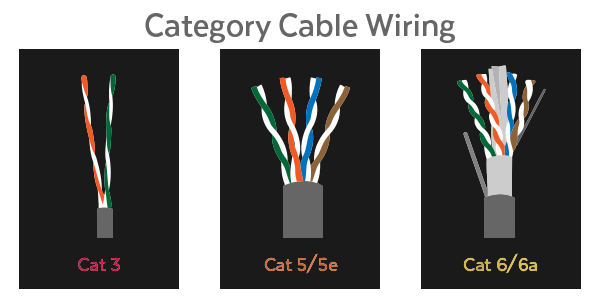
\includegraphics[keepaspectratio = true, width=0.9\textwidth]{figures/category-cable-wiring.png}
				\end{figure}
		\end{frame}

	\subsection{Protocols}
		\begin{frame}
			\frametitle{Pila de protocol per capes}
			\framesubtitle{}
				\begin{itemize}
					\item{Generalment les comunicacions en xarxes es regeixen pel model OSI (Open Systems Interconnection) de ISO}
					\item{Aquest model organitza els protocols per capes: f\'isica, de xarxa, d'aplicaci\'o, \ldots}
					\item{Cada capa rep dades de la inferior i subministra dades a la superior}
				\end{itemize}
				\begin{figure}
					\includegraphics[keepaspectratio = true, width=0.7\textwidth]{figures/ethernet.png}
				\end{figure}
		\end{frame}

		\begin{frame}
			\frametitle{Protocols}
			\framesubtitle{Ethernet}
				\begin{itemize}
					\item{Aquest \'es un protocol senzill, on s'han d'enviar poques dades a m\'es de les que es volen transportar (26 bytes + dades)}
					\item{El pre\`ambul no \'es informaci\'o \'util com a tal, serveix per sincronitzar}
				\end{itemize}
				\begin{figure}
					\includegraphics[keepaspectratio = true, width=0.9\textwidth]{figures/trama_ethernet.png}
				\end{figure}
		\end{frame}

		\begin{frame}
			\frametitle{Protocols}
			\framesubtitle{IPv4}
				\begin{itemize}
					\item{Internet Protocol version 4}
					\item{Protocol b\`asic per dirigir-se als equips d'una xarxa, sigui local o global}
					\item{Imprescindible a la xarxa de xarxes}
					\item{Relativament complicat perqu\`e ha de contemplar gran varietat de casos (fragmentaci\'o, diferents subprotocols, \ldots)}
				\end{itemize}
		\end{frame}

		\begin{frame}
			\frametitle{Protocols}
			\framesubtitle{IPv4}
				\begin{figure}
					\includegraphics[keepaspectratio = true, width=0.65\textwidth]{figures/paquet_ipv4.png}
				\end{figure}
		\end{frame}

		\begin{frame}
			\frametitle{Protocols}
			\framesubtitle{ARP}
				\begin{itemize}
					\item{Address Resolution Protocol}
					\item{Protocol b\`asic per identificar els equips dins d'una xarxa local}
					\item{Complement ideal entre IPv4 i Ethernet per xarxes locals}
				\end{itemize}
		\end{frame}

		\begin{frame}
			\frametitle{Protocols}
			\framesubtitle{ARP}
				\begin{figure}
					\includegraphics[keepaspectratio = true, width=0.375\textwidth]{figures/paquet_arp.png}
				\end{figure}
		\end{frame}

		\begin{frame}
			\frametitle{Protocols}
			\framesubtitle{ICMP}
				\begin{itemize}
					\item{Internet Control Message Protocol}
					\item{Protocol que serveix per regular el tr\`afic, generalment, a la xarxa de xarxes}
					\item{Serveix per notificar de p\`erdua de paquets, comprovar l'estat de la xarxa}
					\item{Es pot utilitzar en xarxes locals per provar la capacitat de la xarxa}
				\end{itemize}
		\end{frame}

		\begin{frame}
			\frametitle{Protocols}
			\framesubtitle{ICMP}
				\begin{figure}
					\includegraphics[keepaspectratio = true, width=0.9\textwidth]{figures/paquet_icmp.png}
				\end{figure}
		\end{frame}

\section{Implementaci\'o pr\`actica}
	\subsection{LwIP}
		\begin{frame}
			\frametitle{Implementaci\'o pr\`actica}
			\framesubtitle{LwIP}
				\begin{itemize}
					\item{LwIP \'es una de les implementacions de TCP/IP m\'es utilitzades}
					\item{Pila espec\'ificament dissenyada per aplicacions incrustades}
					\item{Microcontroladors amb poca mem\`oria de codi (ocupa al voltant de 40 kilobytes per si sola)}
					\item{No necessita de molta mem\`oria RAM, sempre en funci\'o de les demandes de la xarxa i l'aplicaci\'o}
					\item{Pila de protocols molt capa\c c, suporta la majoria de protocols utilitzats a Internet}
				\end{itemize}
		\end{frame}

		\begin{frame}
			\frametitle{Implementaci\'o pr\`actica}
			\framesubtitle{LwIP}
				\lstinputlisting[language = C, morekeywords = {xil_printf, inicialitza_temporitzador, inicialitza_interrupcions, inicialitza_lwip, arrenca_app, xemacif_input, tcp_fasttmr, tcp_slowtmr, Xil_ExceptionEnable}]{codi/lwip_main.c}
		\end{frame}

	\subsection{Sense LwIP}
		\begin{frame}
			\frametitle{Implementaci\'o pr\`actica}
			\framesubtitle{Sense LwIP}
				\begin{itemize}
					\item{Implementaci\'o feta per l'autor}
					\item{Pila de protocols molt redu\"ida: ARP, i ICMP sobre IPv4 (sense fragmentaci\'o)}
					\item{Intent d'optimitzar el m\`axim possible tant la mem\`oria ocupada pel codi com la velocitat d'execuci\'o}
					\item{B\`asicament capa\c c de respondre a peticions d'eco i poc m\'es}
				\end{itemize}
		\end{frame}

		\begin{frame}
			\frametitle{Implementaci\'o pr\`actica}
			\framesubtitle{Sense LwIP}
				\lstinputlisting[language = C, morekeywords = {xil_printf, inicialitza_temporitzador, inicialitza_interrupcions, inicialitza_lwip, inicialitza_emaclite, arrenca_app, xemacif_input, tcp_fasttmr, tcp_slowtmr, Xil_ExceptionEnable, memcpy}]{codi/sense_lwip_main.c}
		\end{frame}

		\begin{frame}
			\frametitle{Implementaci\'o pr\`actica}
			\framesubtitle{Sense LwIP}
				\lstinputlisting[language = C, morekeywords = {xil_printf, inicialitza_temporitzador, inicialitza_interrupcions, inicialitza_lwip, inicialitza_emaclite, arrenca_app, xemacif_input, tcp_fasttmr, tcp_slowtmr, Xil_ExceptionEnable, memcpy}]{codi/sense_lwip_arp.c}
		\end{frame}

		\begin{frame}
			\frametitle{Implementaci\'o pr\`actica}
			\framesubtitle{Sense LwIP}
				\lstinputlisting[language = C, morekeywords = {xil_printf, inicialitza_temporitzador, inicialitza_interrupcions, inicialitza_lwip, inicialitza_emaclite, arrenca_app, xemacif_input, tcp_fasttmr, tcp_slowtmr, Xil_ExceptionEnable, memcpy}]{codi/sense_lwip_icmp.c}
		\end{frame}

\section{Resultats experimentals}
	\subsection{M\`etode d'estudi}
		\begin{frame}
			\frametitle{Resultats experimentals}
			\framesubtitle{M\`etode d'estudi}
				\begin{itemize}
					\item{S'executen gran nombre de peticions d'eco}
					\item{Llarg\`aria de les dades del paquet ICMP variable}
					\item{Automatitzat amb script de bash}
				\end{itemize}
				\lstinputlisting[language = bash, morekeywords={sudo, ping, sleep}]{codi/script.sh}
		\end{frame}

	\subsection{Cablejats diferents}
		\begin{frame}
			\frametitle{Resultats experimentals}
			\framesubtitle{Implementacions sobre cablejats diferents - Cat3}
				\begin{figure}
					\includegraphics[keepaspectratio = true, width=0.9\textwidth]{figures/cat3.pdf}
				\end{figure}
		\end{frame}

		\begin{frame}
			\frametitle{Resultats experimentals}
			\framesubtitle{Implementacions sobre cablejats diferents - Cat6}
				\begin{figure}
					\includegraphics[keepaspectratio = true, width=0.9\textwidth]{figures/cat6.pdf}
				\end{figure}
		\end{frame}

	\subsection{Sumes de verificaci\'o}
		\begin{frame}
			\frametitle{Resultats experimentals}
			\framesubtitle{Sumes de verificaci\'o}
				\begin{figure}
					\includegraphics[keepaspectratio = true, width=0.9\textwidth]{figures/checksums.pdf}
				\end{figure}
		\end{frame}

	\subsection{Mem\`oria d'execuci\'o}
		\begin{frame}
			\frametitle{Resultats experimentals}
			\framesubtitle{Mem\`oria d'execuci\'o}
				\begin{figure}
					\includegraphics[keepaspectratio = true, width=0.9\textwidth]{figures/memories.pdf}
				\end{figure}
		\end{frame}

\section{Conclusions}
\subsection*{}
		\begin{frame}
			\frametitle{Conclusions}
			\framesubtitle{}
		\end{frame}

		\begin{frame}
			\frametitle{M\'es informaci\'o}
			\framesubtitle{}
			\vfill
			M\'es informaci\'o i codi font a:
			\url{https://github.com/markopesevski/TFM}
			\vfill
 		\end{frame}

%------------------------------------------------

\section*{}
\begin{frame}[plain]
	\addtocounter{framenumber}{-1}

	\begin{center}
		{\Huge{Gr\`acies per la vostra atenci\'o}}
	\end{center}
	\begin{center}
		{\large{Dubtes? Comentaris? Preguntes?}}
	\end{center}
\end{frame}

%----------------------------------------------------------------------------------------

\end{document}
